\chapter{Tvorba aplikácie}\label{ch:appCreation}

V tejto kapitole sa budeme venovať postupu riešenia zadanej problematiky. Oboznámime sa s implementáciou a využitím najdôležitejších
častí aplikácie. Popíšeme priebeh testovania počas vývoja a na záver sa zameriame na možnosti rozšírenia do budúcnosti, ktoré
by mohli zlepšiť funkcionalitu aplikácie.

\section{Prístup k problematike}\label{sec:solutionApproach}

Aplikácia je implementovaná v programovacom jazyku Python. Využíva externé knižnice, ako sú Matplotlib pre grafickú vizualizáciu
charakteristík, re pre spracovanie textových dát, NumPy pre numerické výpočty a prácu s dátami, wxPython pre vytvorenie grafického
používateľského rozhrania, NetworkX pre prácu s pozičnou slovnou sieťou, výpočet analýzy.

Prvým krokom bolo získanie textových dát pre analýzu. Na tento účel bola využitá stránka Project Gutenberg \cite{projectgutenberg} ,
kde je možné nájsť množstvo verejne dostupných literárnych diel od rôznych autorov preložených do rôznych svetových jazykov.

Následne bolo nevyhnutné zadefinovať spôsob, akým sa vytvorí pozičná slovná sieť. Každé slovo v texte sa považuje za vrchol,
tvar slova sa významovo nemení, iba sa normalizuje celé slovo na malé písmená. Dva vrcholy sú spojené neorientovanou neohodnotenou
hranou v prípade, že im príslušné slová nasledujú v texte bezprostredne za sebou. Vytvorená sieť je teda neorientovaná a neohodnotená.

Ak je pri tvorbe siete zvolená množina interpunkčných znakov, tieto sa považujú za samostatné slová, ostatné sa zanedbávajú a sieť sa tvorí
rovnakým postupom.

Pri vizualizácii sa zameriame na zobrazenie distribúcie stupňov vrcholov, ktorá je jednou z najdôležitejších charakteristík
pozičnej slovnej siete. Taktiež zobrazíme závislosť veľkosti siete (t.j. počtu vrcholov) od hodnoty exponentu $\gamma$ mocninového zákona.

Výpočet analýzy siete je rozdelený do dvoch oblastí. Prvou je grafová analýza, ktorá sa zaoberá výpočtom základných veličín siete, ako je
počet vrcholov; počet hrán; maximálny, minimálny, priemerný stupeň vrcholov; hustota siete; priemerný koeficient zhlukovania; priemerná
najkratšia cesta; priemer siete a korelácie medzi jednotlivými centralitami. Druhou oblasťou je jazyková analýza, ktorá zahŕňa výpočet
jazykových charakteristík, ako je počet slov; maximálna, minimálna, priemerná dĺžka slova; počet viet; maximálna, minimálna, priemerná dĺžka vety;
počet dvojíc a trojíc slov (frázy), ich frekvencia (maximálna, minimálna, priemerná) a počet interpunkčných znakov vrátane ich najčastejšieho a najmenej
častého výskytu.

Výsledky uvedených grafických a výpočtových analýz budú porovnávané pre dve verzie siete - bez interpunkcie a s interpunkciou. Následne
budeme skúmať ich odlišnosti a podobnosti, taktiež budeme porovnávať výsledky pre rôzne jazyky a rôzne texty.

\section{Grafické používateľské rozhranie}\label{sec:GUI}

Grafické používateľské rozhranie (GUI) je vytvorené pomocou knižnice wxPython. Jeho úlohou je poskytnúť používateľovi
jednoduchý a prehľadný spôsob interakcie s aplikáciou. Obsahuje jednu hlavnú obrazovku, ktorá je rozdelená na niekoľko komponentov,
kde každý z nich má svoju špecifickú funkciu.

Prvý komponent v hornej časti obrazovky je textové pole spolu s tlačidlom, ktoré slúži na načítanie textového súboru.
Po stlačení tlačidla sa otvorí dialógové okno, v ktorom si používateľ môže vybrať textový súbor, ktorý chce analyzovať.
Ako náhle je súbor vybraný, jeho názov sa zobrazí v textovom poli.

Nasleduje rozbaľovacia ponuka, ktorá slúži na výber jazyka textu. Používateľ si môže vybrať z niekoľkých jazykov,
ktoré aplikácia podporuje. Na základe výberu jazyka sa prispôsobia ďalšie nastavenia aplikácie.

Ďalší komponent obsahuje zaškrtávacie políčka na výber interpunkčných znakov, ktoré sa majú
zohľadniť pri tvorbe siete. Obsahuje možnosť označiť všetky interpunkčné znaky naraz alebo ich všetky zrušiť.

V strednej časti obrazovky sa nachádza dialógové pole, ktoré zobrazuje aktuálny stav aplikácie. Tu sa zobrazujú informácie o načítanom súbore,
jazyku, vybraných interpunkčných znakoch a po výpočte analýzy aj výsledky.

Ako posledné obsahuje súbor tlačidiel jednotlivých funkcií aplikácie. Používateľ si môže vybrať, či chce vypočítať analýzu siete,
zobraziť distribúciu stupňov vrcholov, rastovú analýzu siete alebo porovnanie slovnej siete bez interpunkcie so zvolenou sieťou.
Jednou z možností je aj uloženie zvolenej siete do súboru.
Ukážku grafického používateľského rozhrania možno vidieť na obrázku č. \ref{obr:gui}.

\begin{figure}
    \centerline{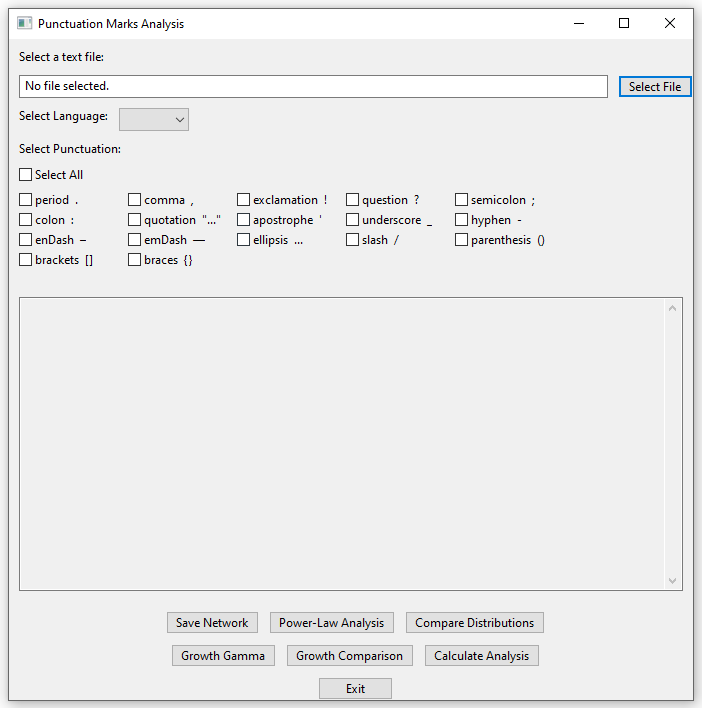
\includegraphics[width=0.8\textwidth]{images/gui.png}}
    \caption[Grafické používateľské rozhranie aplikácie.]{Grafické používateľské rozhranie aplikácie.}
    \label{obr:gui}
\end{figure}
 

\section{Tvorba slovnej siete}\label{sec:creationOfWordNetwork}

Pre vytvorenie slovnej siete je nevyhnutné najprv načítaný textový súbor predspracovať. Cieľom predspracovanie je
vytvorenie normalizovaného zoznamu slov, ktoré budú predstavovať vrcholy siete. Na tento účel sa využíva knižnica \texttt{re},
pretože umožňuje efektívne spracovanie textu pomocou regulárnych výrazov. Vďaka nej možno jednoducho definovať, ktoré
interpunkčné znaky sa majú zohľadniť pri vytváraní siete, a ktoré sa majú ignorovať. 
Metódu predspracovania textu možno vidieť na ukážke č. \ref{lst:textPreprocessing}. Vstupný parameter tejto metódy je
množina interpunkčných znakov, zvolených používateľom prostredníctvom GUI v podobe slovníka, ktorý obsahuje názov
interpunkčného znaku ako kľúč a regulárny výraz ako hodnotu.

\begin{lstlisting}[caption={Metóda predspracovania textu.}, label={lst:textPreprocessing}]
    def processTextFile(self, selectedPunctuation={}):
        if self.selectedLanguage == 'English':
            regexDict = self.regexDictEng
        if self.selectedLanguage == 'German':
            regexDict = self.regexDictGer
        if not selectedPunctuation:
            regexPattern = regexDict['wordsNumbers']
        else:
            usePunctuation = [regexDict[key] for key in selectedPunctuation.keys()]
            regexPattern = '|'.join([regexDict['wordsNumbers']] + usePunctuation)
        data = re.findall(regexPattern, 
                          self.readTextFile(self.inputTextFile))
        if not data:
            return []
        return [word.lower() for word in data]
\end{lstlisting}

Po úspešnom predspracovaní textu sa vytvorí slovník susedností a slovník početností pomocou metódy \texttt{createGraphData}, ktorú
možno vidieť na ukážke č. \ref{lst:createGraphData}. Na reprezentáciu pozičnej slovnej siete sa využíva knižnica \texttt{NetworkX}, špecificky
trieda \texttt{Graph}. Implementáciu je možné vidieť na ukážke č. \ref{lst:networkxGraph}. Naďalej sa pracuje s touto inštanciou triedy \texttt{Graph},
pretože poskytuje množstvo užitočných funkcií a metód na analýzu a vizualizáciu grafov.

\clearpage

\begin{lstlisting}[caption={Metóda pre vytvorenie pozičnej slovnej siete z predspracovaného textu.}, label={lst:createGraphData}]
    def createGraphData(self, data):
        if self.selectedLanguage == 'English':
            regexDict = self.regexDictEng
        if self.selectedLanguage == 'German':
            regexDict = self.regexDictGer
        graphDataDict = {}
        nodeCounter = Counter()
        previousWord = None
        for element in data:
            if element in regexDict['quotation']:
                element = '"'
            if element in regexDict['apostrophe']:
                element = '\''
            if element not in graphDataDict:
                graphDataDict[element] = []
            if previousWord is not None:
                graphDataDict[previousWord].append(element)
                graphDataDict[element].append(previousWord)
            previousWord = element
            nodeCounter[element] += 1
        return graphDataDict, nodeCounter
\end{lstlisting}

\begin{lstlisting}[caption={Vytvorenie inštancie triedy NetworkX.Graph.}, label={lst:networkxGraph}]
    graphData, occurrenceData = self.createGraphData(
            self.processTextFile(self.selectedPunctuation))
        G = nx.Graph()
        for node, neighbors in graphData.items():
            for neighbor in neighbors:
                G.add_edge(node, neighbor)
\end{lstlisting}

\section{Zobrazenie výstupných charakteristík}\label{sec:graphicalOutput}

Na zobrazenie výstupných charakteristík sa využíva knižnica \texttt{Matplotlib}. Táto knižnica poskytuje množstvo funkcií
a metód na vytváranie grafov a vizualizáciu dát. V tejto aplikácii sa budeme zameriavať na zobrazenie distribúcie stupňov
vrcholov, rastovú závislosť siete od hodnoty exponentu $\gamma$ mocninového zákona.

\subsection{Logaritmické zhlukovanie}\label{sec:logarithmicClustering}

Pri vizualizácii distribúcie stupňov vrcholov sa využíva metóda logaritmického zhlukovania, ktorá je implementovaná
v metóde \texttt{calculateLogBin}, ukážka č. \ref{lst:logarithmicClustering}. Táto metóda zhlukuje dáta do logaritmických intervalov,
čo umožňuje lepšie zobrazenie distribúcie stupňov vrcholov v prípade, že sú dáta rozptýlené na širokom intervale hodnôt.

Funkcia najprv vypočíta rozsah stupňov vrcholov, následne vytvorí logaritmicky rozdelené intervaly pomocou funkcie \texttt{np.logspace},
potom vypočíta hustotu pravdepodobnosti pre každý interval pomocou funkcie \texttt{np.histogram}. Výsledkom sú stredy intervalov a
hustoty pravdepodobnosti, ktoré sú následne vrátené ako výstup metódy.

\begin{lstlisting}[caption={Metóda pre výpočet logaritmického zhlukovania.}, label={lst:logarithmicClustering}]
    def calculateLogBin(self, degrees, binCount):
        minDegree = max(1, min(degrees))
        maxDegree = degrees.max()
        bins = np.logspace(np.log10(minDegree), 
                            np.log10(maxDegree), num=binCount)
        hist, binEdges = np.histogram(degrees, bins=bins, 
                                      density=True)
        binCenters = (binEdges[:-1] + binEdges[1:]) / 2
        nonzero = hist > 0
        return binCenters[nonzero], hist[nonzero]
\end{lstlisting}

Výsledné dáta sú zobrazované v log-log grafe, ktorý umožnuje overiť, či dáta nasledujú mocninový zákon a vypočítať hodnotu exponentu
$\gamma$.

\subsection{Distribúcia stupňov vrcholov}\label{sec:degreeDistribution}

Distribúcia stupňov vrcholov udáva, ako sú stupne vrcholov rozložené v sieti. Najskôr sa vypočíta tzv. surová distribúcia stupňov,
ktorá predstavuje relatívny výskyt každého stupňa v sieti. Pri slovnej sieti býva táto distribúcia zvyčajne veľmi rozptýlená,
preto je ťažké získať prehľad o tom, ako sú stupne vrcholov rozložené. Z toho dôvodu sa používa logaritmické zhlukovanie \ref{sec:logarithmicClustering},
ktoré zoskupuje dáta do logaritmických intervalov. Porovnanie surovej distribúcie stupňov vrcholov s logaritmicky zhlukovanou distribúciou stupňov
vrcholov je zobrazené na obrázku č. \ref{obr:rawLogBinnedDegDist}.

Práve logaritmicky zhlukovaná distribúcia stupňov vrcholov je veľmi dôležitá pre analýzu siete, pretože sa využíva na porovnanie
s teoretickým mocninovým rozdelením. Pomocou tejto metódy vizualizácie je možné vypočítať hodnotu exponentu $\gamma$ mocninového zákona, ktorý
udáva, ako sú stupne vrcholov rozložené v sieti.

\clearpage

\begin{figure}
    \centerline{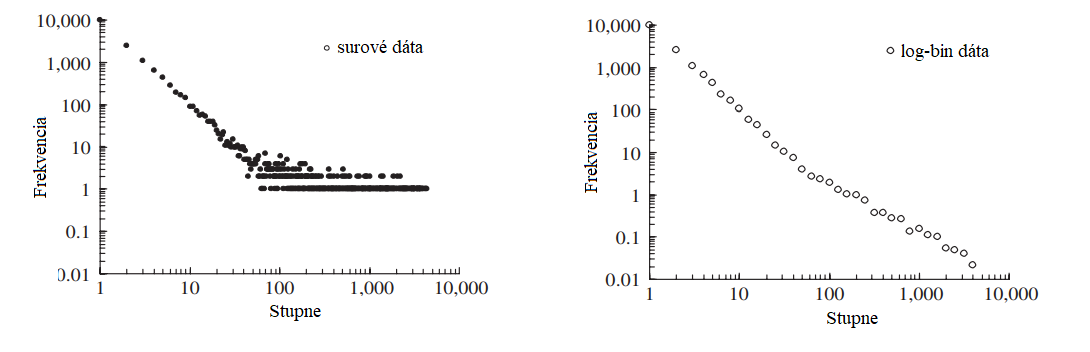
\includegraphics[width=1\textwidth]{images/rawLogBinnedDegDist.png}}
    \caption[Distribúcia stupňov vrcholov bez a s pomocou logaritmického zhlukovania.]{Distribúcia stupňov vrcholov bez a s pomocou logaritmického zhlukovania \cite{milojevic2010power}.}
    \label{obr:rawLogBinnedDegDist}
\end{figure}

\subsection{Rastová analýza siete}\label{sec:growthAnalysis}

Rastová analýza siete je ďalšou dôležitou charakteristikou, ktorá sa zaoberá tým, ako sa mení štruktúra siete pri zmene veľkosti textu. V tejto analýze
sa skúma, ako sa vyvíja hodnota exponentu $\gamma$ mocninového zákona v závislosti od veľkosti siete (počtu vrcholov). 
Takáto analýza nám umožňuje určiť, pri akej veľkosti textu sa hodnota exponentu $\gamma$ stabilizuje, tým pádom vieme určiť, akú veľkosť textu je potrebné
použiť na získanie reprezentatívnych výsledkov.

Postup spočíva v rozdelení textu na rovnomerné časti, z ktorých sa vytvára sieť. Pre každú z týchto sietí sa vypočíta logaritmicky zhlukovaná distribúcia stupňov vrcholov
a následne sa určí hodnota exponentu $\gamma$. Výsledkom je graf, ktorý zobrazuje hodnotu exponentu $\gamma$ v závislosti od počtu vrcholov v sieti, zobrazený na obrázku č. \ref{obr:growthPlot}.

\begin{figure}
    \centerline{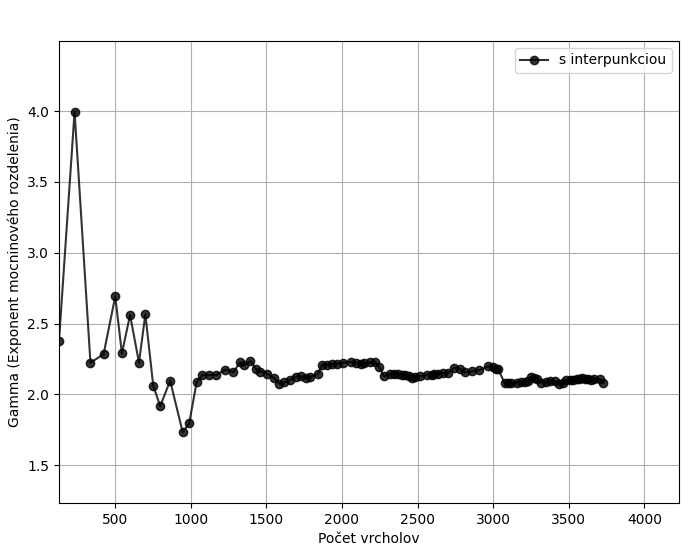
\includegraphics[width=0.8\textwidth]{images/growthPlot.png}}
    \caption[Rastová charakteristika, hodnota exponentu $\gamma$ v závislosti od počtu vrcholov v sieti.]{Rastová charakteristika, hodnota exponentu $\gamma$ v závislosti od počtu vrcholov v sieti.}
    \label{obr:growthPlot}
\end{figure}

\section{Výpočet analýzy siete}\label{sec:calculationOfNetworkAnalysis}

Výpočet analýzy siete je rozdelený do dvoch oblastí. Prvá, grafická analýza je implementovaná pomocou zadefinovaných
metód v knižníci \texttt{NetworkX}. Druhá, jazyková analýza je implementovaná pomocou vlastných metód,
ktoré sú špecifické pre danú aplikáciu.

\section{Uloženie siete do súboru}\label{sec:savingNetworkToFile}

Jednou z funkcionalít aplikácie je uloženie vytvorenej slovnej siete do súboru. Na tento účel sa využíva knižnica \texttt{NetworkX},
ktorá poskytuje metódy na exportovanie grafov do rôznych formátov. V tejto aplikácii sa využíva formát \texttt{GraphML}, ktorý je
vhodný pre externé aplikácie na analýzu a vizualizáciu grafov, ako \texttt{Cytoscape} \cite{cytoscape_website}
alebo \texttt{Gephi} \cite{gephi_website}. 

Uloženie siete do súboru je implementované v metóde \texttt{saveNetwork}, ktorú možno
vidieť na ukážke č. \ref{lst:saveNetwork}. Táto metóda sa volá po stlačení tlačidla "Save Network" v GUI, ktontroluje či je vybraná
interpunkcia a následne uloží sieť do súboru s názvom, ktorý je odvodený od názvu vstupného textového súboru a vypíše miesto uloženia
do dialógového okna.

\begin{lstlisting}[caption={Uloženie siete do súboru.}, label={lst:saveNetwork}]
    def saveNetwork(self, event):
        self.logMessage(self.collectInputDataInfo())
        self.logMessage('Saving network...\n')

        N = nx.Graph(self.createGraphData(
                self.processTextFile(self.selectedPunctuation))[0])
        if self.selectedPunctuation:
            graphName = f'{self.labelFileSelectPath.GetValue().split('/')[-1].split('.')[0]}_graphYesPunct.graphml'
            self.logMessage(f'Saving graph to {graphName}')
            nx.write_graphml(N, f'{graphName}')
        else:
            graphName = f'{self.labelFileSelectPath.GetValue().split('/')[-1].split('.')[0]}_graphNoPunct.graphml'
            self.logMessage(f'Saving graph to {graphName}')
            nx.write_graphml(N, graphName)
\end{lstlisting}


\section{Testovanie}\label{sec:testing}

Testovanie aplikácie bolo vykonané v niekoľkych fázach počas vývoja. Cieľom bolo zabezpečiť správnu funkcionalitu jednotlivých
komponentov a výstupov aplikácie. Testovanie prebiehalo prevažne manuálne s využitím jednoduchých testovacích skriptov
a simulácií rôznych vstupných dát.

\subsection{Testovanie predspracovania textu a vytvorenia slovnej siete}\label{sec:testingPreprocessing}

Prvou fázou testovania bolo testovanie korektnosti a funkčnosti predspracovania textu a vytvorenia slovnej siete. Pomocou jednoduchých
testovacích skriptov a simulácie rôznych vstupných dát sa overovalo:
\begin{itemize}
    \item Správnosť predspracovania textu (rozdelenie textu na slová)
    \item Správnosť zohľadnenia interpunkčných znakov pri predspracovaní textu (ak boli zvolené interpunkčné znaky)
    \item Správnosť vytvorenia slovnej siete
    \item Správnosť počtu vrcholov a hrán v sieti
    \item Správnosť reprezentácie siete pomocou knižnice NetworkX
\end{itemize}

\subsection{Testovanie grafického používateľského rozhrania}\label{sec:testingGUI}

Funkcionalita grafického používateľského rozhrania bola testovaná manuálne. Overovala sa:
\begin{itemize}
    \item Funkčnosť tlačidiel (načítanie textového súboru, uloženie siete, zobrazovanie a výpočet analýz)
    \item Funkčnosť rozbaľovacej ponuky pre výber jazyka
    \item Funkčnosť zaškrtávacích okien pre výber interpunkčných znakov
    \item Funkčnosť dialógového okna (výpis informácií o aktuálnom stave aplikácie)
\end{itemize}

\subsection{Testovanie analýzy siete}\label{sec:testingNetworkAnalysis}

Testovanie vizualizácie charakteristík a výpočtovej analýzy siete bolo vykonané manúalne a na rôznych textoch a jazykoch. Overovalo sa:
\begin{itemize}
    \item Správnosť výpočtu základných grafových veličín siete (overenie správnosti výstupov pomocou externého nástroja \texttt{Cytoscape} \cite{cytoscape_website} )
    \item Správnosť výpočtu jazykových charakteristík siete (overenie správnosti výstupov na simulovaných textoch)
    \item Správnosť zobrazenia distribúcie stupňov vrcholov
    \item Správnosť zobrazenia rastovej analýzy siete
    \item Konzistentnosť výsledkov pri rôznych vstupoch
    \item Odozva pri rozdielnych veľkostiach vstupných textov
\end{itemize}


\section{Možnosti budúceho rozšírenia}\label{sec:futureExtensions}

V tejto časti sa zameriame na potenciálne možnosti vylepšenia a rozšírenia aplikácie, ktoré by mohli zlepšiť funkcionalitu
a použiteľnosť aplikácie pri analýze textových dát. Tieto vylepšenia by mohli zahŕňať:
\begin{itemize}
    \item Podporovanie viacerých jazykov a textových formátov
    \item Načítanie slovnej siete zo súboru
    \item Možnosť manuálneho nastavenia parametrov pri charakteristikách, ako je veľkosť výseku vstupného textu alebo dĺžka najdlhšej
    klesajúcej sekvencie vrcholov
    \item Manuálne nastavenie parametrov pre logaritmické zhlukovanie, aby používateľ mohol získať presnejšie
    výsledky pre konkrétne texty
    \item Výber veličín, ktoré sa majú vypočítať a zobraziť pri analýze siete
    \item Možnosť porovnávať viacero rôznych sietí naraz a zobraziť ich výsledky v jednom grafe
    \item Možnosť uloženia siete, grafov v rôznych formátoch

\end{itemize}